% kuleuventheme2 by Janez Kren, September 2017, janez.kren@kuleuven.be, based on:
% kuleuventheme 1.3 by Roland Pastorino, 2013 roland.pastorino@kuleuven.be / www.rolandpastorino.com

\documentclass[11pt,t]{beamer}
\usetheme{kuleuven2}	%THEME OPTIONS for LOGO: kul (default), kulak, lrd,    ; OPTIONS for TITLE PAGE: normal (default), sedes


%%% OTHER SETTINGS
\usefonttheme[onlymath]{serif}			% math font with serifs, delete to make it sans-serif
\setbeamertemplate{footline}[body] 		% delete this line to remove footline bar on all frames
%\usepackage[orientation=landscape,size=custom,width=16,height=9,scale=0.5,debug]{beamerposter} %enable for widescreen 16:9 ratio
%\titlegraphic{ \includegraphics[width=.2\paperwidth]{mytitlepagepic.png} } %optional title page image


%%% ADDED PACKAGES:
\usepackage[english]{babel}
\usepackage{amsfonts}
\usepackage{amssymb}
\usepackage{amsmath}


%%% TITLE PAGE INFO:
\title[Midterm presentation]{Avoiding local minima in Deep Learning: a nonlinear optimal control approach} %[]] will appear in footline
\subtitle{Midterm presentation}

\author{Jan Scheers \\
Promotor: Prof. Panos Patrinos \\
Supervisors: Masoud Ahookhosh, Andreas Themelis}
\date{December 2018}




\begin{document}
\csname beamer@calculateheadfoot\endcsname %recalculate head and foot dimension


 %%
 %%  0. TITLE PAGE and TABLE OF CONTENT
 %%
% Title page
\begin{frame}[plain,noframenumbering]
	\titlepage
\end{frame}

\section{Neural Networks}

\begin{frame}{Neural Networks and Deep Learning}
   \begin{itemize}
      \itemsep 15pt
      \item Very popular these days
      \item Very expressive / low bias
      \item Good for big data sets/unlabeled data sets
      \item Can detect complex nonlinear relationships
      \item Focus on deep feedforward neural networks in this thesis
   \end{itemize}
\end{frame}

\begin{frame}{Neural Network}
   \begin{figure}
	\centering
	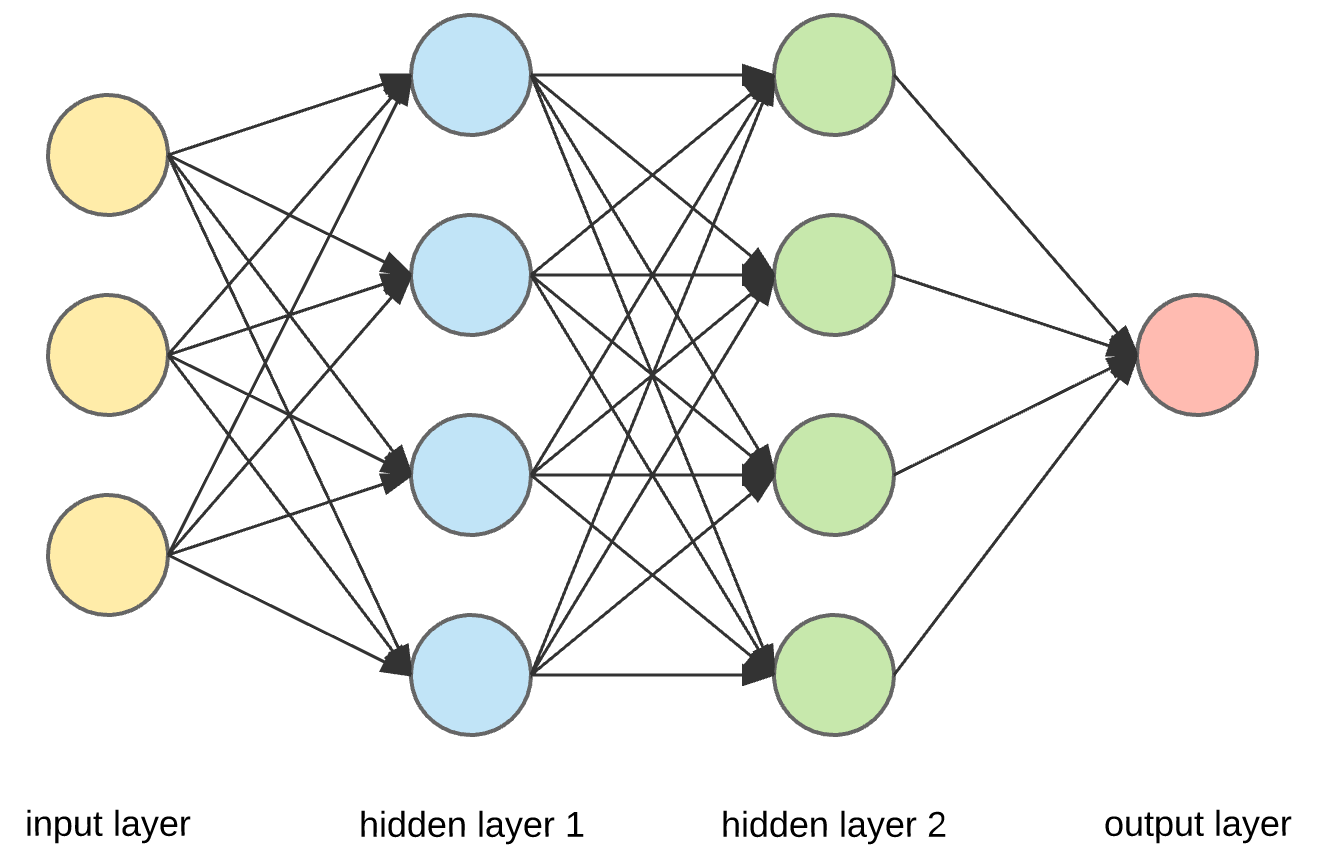
\includegraphics[width=0.7\textwidth]{network}
	\caption{Feedforward Deep Neural Network. (Retrieved from https://towardsdatascience.com, 2018)}
	\end{figure}
\end{frame}


\begin{frame}{Neuron}
\begin{figure}
	\centering
	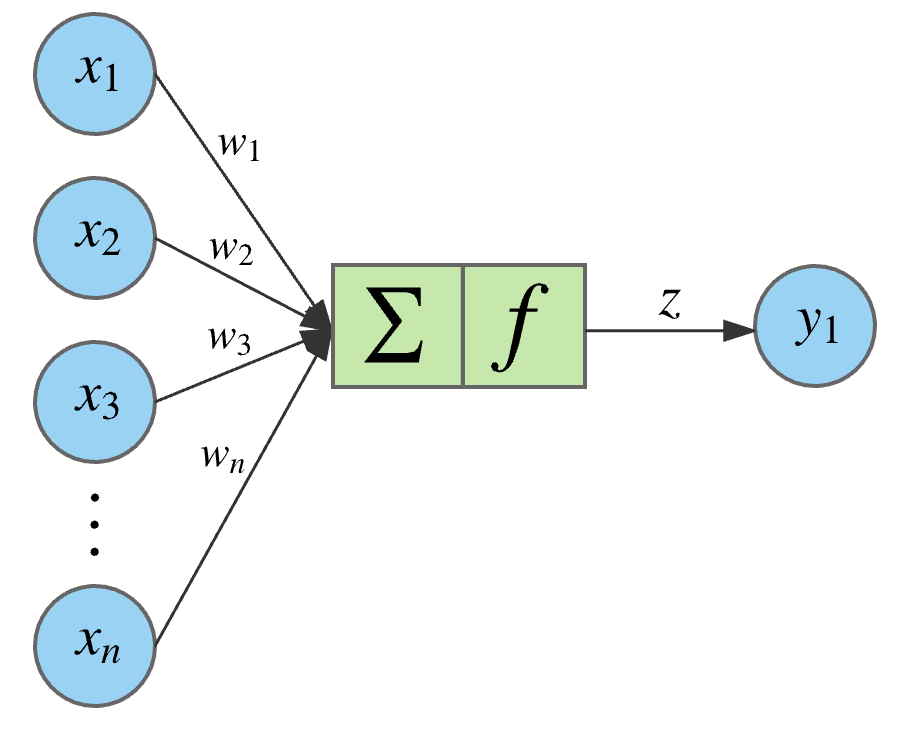
\includegraphics[width=0.6\textwidth]{neuron}
	\caption{Single Neuron - McCulloch–Pitts model. (Retrieved from https://towardsdatascience.com, 2018)}
	\end{figure}
\end{frame}

\begin{frame}{Activation Function}
   \begin{itemize}
      \item McCulloch–Pitts neuron model
      \begin{equation*}
      y = \sigma(w_1x_1+w_2x_2+...+w_nx_n)
      \end{equation*}
      \item Rectified Linear Unit (ReLU)
      \begin{equation*}
      \sigma(x) = x^+ = \max(0,x)
      \end{equation*}
      \item Most commonly used activation function
      \begin{figure}
	   \centering
	   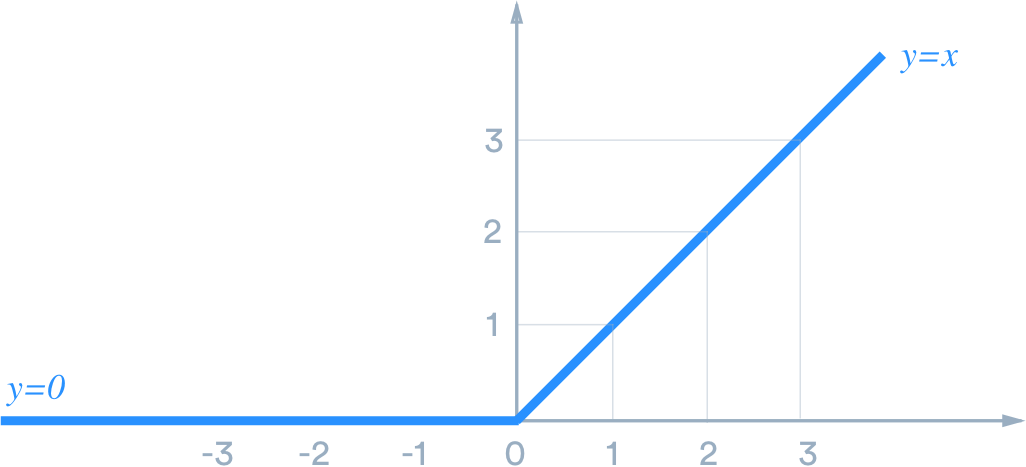
\includegraphics[height=0.3\textheight]{relu}
	   %%\caption{Example graphic \label{fig:figure1}}
	   \end{figure}
   \end{itemize}

\end{frame}

\begin{frame}{Training}
   \begin{itemize}
      \item Matrix notation of network
      \begin{equation*}
         f(W,x) = W_H\sigma(W_{H-1}\sigma(...W_1\sigma(W_0x)...))
      \end{equation*}
      \item Training of neural network optimizes cost function for dataset

      \begin{equation*}
      \begin{aligned}
      & \underset{W}{\text{minimize}}
      & L(W) &= \sum\limits_{j=0}^{N}||f(W,x^j) - y^j||^2 \\
      \end{aligned}
      \end{equation*}

      \item Usual algorithm is backpropagation
      
      \begin{itemize}
         \item Calculate output of network
         \item Propagate error backwards
         \item Calculate gradient
      \end{itemize}
   \end{itemize}
\end{frame}

\section{Neural Networks as Dynamical Systems}

\begin{frame}{Neural Network as Dynamical System}
   \begin{itemize}
      \item Matrix notation of network
      \begin{equation*}
         f(W,x) = W_H\sigma(W_{H-1}\sigma(...W_1\sigma(W_0x)...))
      \end{equation*}


      \item As a dynamical system
      \begin{equation*}
      \begin{aligned}
      x_0 &= x \\
      x_{k+1} &= \sigma(W_kx_k), & k = 0,...,H-1 \\
      y &= W_Hx_H \\
      \end{aligned}
      \end{equation*}
      \item Every layer is a state
      \item Weight matrices are inputs


   \end{itemize}
\end{frame}

\begin{frame}{Linear Neural Networks}
   \begin{itemize}
      \item Matrix notation
      \begin{equation*}
      \begin{aligned}
      & \underset{W}{\text{minimize}}
      & & L(W) = ||W_HW_{H-1}\ldots W_1X - Y||^2 \\
      \end{aligned}
      \end{equation*}
      
      \item Proof exists that these networks have no bad local minima (Kawaguchi, 2017)\cite{DBLP:journals/corr/LuK17}
      
      \item System Equations
      \begin{equation*}
      \begin{aligned}
      x_0 &= x \\
      x_{k+1} &= W_kx_k, & k = 0,...,H-1 \\
      y &= W_Hx_H \\
      \end{aligned}
      \end{equation*}
      
      \item Objective: recreate proof using dynamical system interpretation
      
   \end{itemize}
\end{frame}

\begin{frame}{Linear Neural Network Proof Problems}

   \begin{itemize}
      
      \item Even though network is linear, system is nonlinear
      \item Inputs and states are not separated
      \item Understood previous proof
      \begin{itemize}
         \item Did not help much in formulating new proof
      \end{itemize}
      
      \item System Equations
      \begin{equation*}
      \begin{aligned}
      x_0 &= x \\
      x_{k+1} &= W_kx_k, & k = 0,...,H-1 \\
      y &= W_Hx_H \\
      \end{aligned}
      \end{equation*}
      
      $\Rightarrow$ Change objective to training networks using Control Theory
   \end{itemize}

\end{frame}

\section{Training as Optimal Control Problem}

\begin{frame}{Training as Optimal Control Problem}
   \begin{itemize}
   \item Training a network with ReLU activation functions is equivalent to following Optimal Control Problem (OCP)
      \begin{equation*}
      \begin{aligned}
      & \underset{W}{\text{minimize}}
      & & \sum\limits_{j=0}^{N}||W_Hx_H^j - y^j||^2 \\
      & \text{subject to}
      & & x_{k+1}^j = \max(W_kx_k^j,0), &k = 0,\ldots,H-1,j = 1,\ldots,N
      \end{aligned}
      \end{equation*}
   \end{itemize}
\end{frame}

\begin{frame}{Transforming ReLU Constraints}
   \begin{gather*}
   x_{k+1}^j = \max(W_kx_k^j,0) \\
   \Updownarrow \\
   x_{k+1}^j = -\min(-W_kx_k^j,0) \\
   \Updownarrow \\
   \min(x_{k+1}^j-W_kx_k^j) = 0 \\
   \Updownarrow \\
   (x_{k+1}^j-W_kx_k^j)^\top x_{k+1}^j = 0,\\
   x_{k+1}^j\geq 0,x_{k+1}^j-W_kx_k^j\geq 0
   \end{gather*}
   
   $\Rightarrow$ Now constraint function is smooth
\end{frame}

\begin{frame}{Solving the OCP}
   \begin{itemize}
   \item Problem formulation with relaxed constraints
      \begin{equation*}
      \begin{aligned}
      & \underset{W}{\text{minimize}}
      & & \sum\limits_{j=0}^{N}||W_Hx_H^j - y^j||^2 \\
      & \text{subject to}
      & & (x_{k+1}^j-W_kx_k^j)^\top x_{k+1}^j {\boldsymbol\leq} 0, &k = 0,\ldots,H-1,j = 1,\ldots,N \\
      & & & x_{k+1}^j\geq 0,x_{k+1}^j-W_kx_k^j\geq 0, &k = 0,\ldots,H-1,j = 1,\ldots,N
      \end{aligned}
      \end{equation*}
   \end{itemize}
\end{frame}

\begin{frame}{Solving the OCP}
   \begin{itemize}
   \itemsep 10pt
   \item Two ways of transforming OCP to standard optimization problem
   \item Sequential approach: eliminate states using dynamics
   \begin{itemize}
      \vspace{5pt}
      \itemsep 5pt
      \item This is Backpropagation algorithm
      \item Standard approach for training networks
   \end{itemize}
   \item Simultaneous approach: Keep states as variables, dynamics as constraints
   \begin{itemize}
      \vspace{5pt}
      \itemsep 5pt
      \item Often works better for highly nonlinear problems
      \item Novel approach for Neural Networks
      \item Topic of thesis
   \end{itemize}
   \end{itemize}
\end{frame}

\begin{frame}{Penalty Method}
   \begin{itemize}
      \item Penalty method is simplest
      \item Take constrained problem
      \begin{equation*}
      \begin{aligned}
      & \underset{x}{\text{min}}
      & & f(x) \\
      & \text{s.t.}
      & & g_i(x) \leq 0, & i = 1,\ldots,m \\
      \end{aligned}
      \end{equation*}
      \item Solve series of unconstrained problems
      \begin{equation*}
      \begin{aligned}
      & \underset{x}{\text{min}} 
      & & \Phi_k(x) = f(x) + \sigma_k \sum\limits_{i} \max(0,g_i(x))^2   \\
      \end{aligned}
      \end{equation*}
      \item In each iteration increase size of penalty parameter $\sigma_k$
   \end{itemize}
\end{frame}

\begin{frame}{Augmented Lagrangian Method}
   \begin{itemize}
      \item Similar to penalty method
      \item For constrained problem
      \begin{equation*}
      \begin{aligned}
      & \underset{x}{\text{min}}
      & & f(x) \\
      & \text{s.t.}
      & & g_i(x) \leq 0, & i = 1,\ldots,m \\
      \end{aligned}
      \end{equation*}
      \item Add Langrange multipliers
      \item Solve series of unconstrained problems
      \begin{equation*}
      \begin{aligned}
      & \underset{x}{\text{min}} 
      & & \Phi_k(x) = f(x) + \frac{\sigma_k}{2} \sum\limits_{i} \max(0,g_i(x))^2 - \sum\limits_{i}\lambda_ig_i(x)   \\
      \end{aligned}
      \end{equation*}
      \item In each iteration increase size of penalty parameter $\sigma_k$ and update Lagrange parameters $\lambda_i$
      
   \end{itemize}
\end{frame}

\begin{frame}{Comparison to Backpropagation}
   \begin{itemize}
      \itemsep 15pt
      \item Including states as variables increases problem size greatly
      \item Problem becomes less nonlinear
      \item In Optimal Control Problems simultaneous approach usually better then sequential approach when problem is highly nonlinear
      \item Might be easier to parallellize
   \end{itemize}
\end{frame}

\section{Future Work}
\begin{frame}{Planning of Future Work}
   \begin{itemize}
   \itemsep 10pt
   \item Explore Penalty Method and Augmented Lagrangian Method compared to Backpropagation
   \item In Matlab
   \item If promising, switch to language such as C++/Fortran
   \item Maybe explore other optimization methods
   \item Explore Online/Offline training
   \item \ldots
   \end{itemize}
   %\cite{BertsekasDimitriP1999Np}
\end{frame}

\section{References}

\begin{frame}{References}
%\cite{BertsekasDimitriP1999Np}\cite{NocedalJorge2006No}

\bibliography{all.bib}{}
\bibliographystyle{abbrv}
\end{frame}


\begin{frame}[c,plain,noframenumbering]
\begin{tikzpicture}[remember picture,overlay]
\fill[fill=kul-blue]
    (current page.south east)  rectangle  ([shift={(0,-0.1\paperheight)}]current page.north west)   ;
\end{tikzpicture}

\centering
\textcolor{white}{\huge Questions?}
\end{frame}

\end{document}